\documentclass[12pt]{article}
\usepackage[utf8]{inputenc}
\usepackage{amsmath}
\usepackage{listings}
\usepackage{color}
\usepackage{babel,blindtext}
\usepackage{caption}
\usepackage{subcaption}
\usepackage{float}
\usepackage{graphicx}
\graphicspath{ {./images/} }
\definecolor{dkgreen}{rgb}{0,0.6,0}
\definecolor{gray}{rgb}{0.5,0.5,0.5}
\definecolor{mauve}{rgb}{0.58,0,0.82}
\linespread{1.1}

\lstset{frame=tb,
  language= MATLAB,
  aboveskip=3mm,
  belowskip=3mm,
  showstringspaces=false,
  columns=flexible,
  basicstyle={\small\ttfamily},
  numbers=none,
  numberstyle=\tiny\color{gray},
  keywordstyle=\color{blue},
  commentstyle=\color{dkgreen},
  stringstyle=\color{mauve},
  breaklines=true,
  breakatwhitespace=true,
  tabsize=3
}
\title{CSC336 A3}
\author{Yichen Ji }
\date{April 2021}

\begin{document}

\maketitle

\section{Q1}

(a)

First write the system in the standard form $\bar{f}(\bar{x}^{(i)})=\bat{0}$, that is, 
\begin{align}
\bar{f} &=
\begin{bmatrix}
f_1(\bar{x}^{(i)}) \\
f_2(\bar{x}^{(i)})\\
f_3(\bar{x}^{(i)})\\
f_4(\bar{x}^{(i)})\\
f_5(\bar{x}^{(i)})\\
\end{bmatrix}
&= 
\begin{bmatrix}
(1+h\mu+h\rho)x_1^{(i)}+h\frac{\beta}{N}x_1^{(i)}x_3^{(i)}-x_1^{(i-1)}-h \mu N\\
(1+h\alpha+h\mu)x_2^{(i)}-h\frac{\beta}{N}x_1^{(i)}x_3^{(i)}-x_2^{(i-1)}\\
-h\alpha x_2^{(i)}+(1+h\gamma+h\mu)x_3^{(i)}-x_3^{(i-1)}\\
-h\gammax_3^{(i)}+(1+h\mu)x_4^{(i)}-x_4^{(i-1)}\\
-h\rho x_1^{(i)}(1+h\mu)x_5^{(i)}-x_5^{(i-1)}\\
\nonumber
\end{bmatrix}
\end{align}

After calculation by hand, the Jacobian matrix for this system is 

\begin{bmatrix}
1+h\mu+h\rho+h\frac{\beta}{N}x_3^{(i)} & 0 & h\frac{\beta}{N}x_1^{(i)} & 0 & 0\\
-h\frac{\beta}{N}x_3^{(i)} & 1+h\alpha+h\mu & -h\frac{\beta}{N}x_1^{(i)} & 0 & 0\\
0 & -h\alpha & 1+h\gamma+h\mu & 0 & 0\\
0 & 0 & -h\gamma & 1+h\mu & 0\\
-h\rho & 0 & 0 & 0 & 1+h\mu \\
\end{bmatrix}

(b)

The MATLAB \textbf{script} is written as follows:
\begin{lstlisting}
% computing the spreading of influenza
% test for Newton's on one (large) timestep

% beta transmission, gamma recovery, mu death/birth (replenishment)
alpha = 1/6; beta = 0.25; gamma = 0.06; mu = 0.01/365; rho = 300*mu;
%rho = 0;

% initial conditions
N = 38e6; y02 = 20e3; y03 = 30e3; y04 = 850e3;
y0 = [N-y02-y03-y04 y02 y03 y04 0]';

dt = 1/2; % stepsize for time is h (or dt)
Alpha = dt*alpha;
Beta = dt*beta/N; 
Gamma = dt*gamma; 
Mu = dt*mu; 
Rho = dt*rho; % for convenience

maxit = 10; tol = 1e-6; % Newton's parameters
fprintf(' k   S         E      I       R          V     Total     Residual\n');
y = y0;
yinit = y; % initial guess for Newton's
for k = 1:maxit
    % define vector f and its inf norm
    f = [(1+Mu+Rho)*y(1)+Beta*y(1)*y(3)-yinit(1)-Mu*N;
        (1+Alpha+Mu)*y(2)-Beta*y(1)*y(3)-yinit(2);
        -Alpha*y(2)+(1+Gamma+Mu)*y(3)-yinit(3);
        -Gamma*y(3)+(1+Mu)*y(4)-yinit(4);
        -Rho*y(1)+(1+Mu)*y(5)-yinit(5)];
    fnorm =max(abs(f));
    fprintf('%2d %10.0f %6.0f %6.0f %9.0f %6.0f %10.0f %9.2e\n', ...
            k-1, y, sum(y), fnorm);
    % stopping criterion
    if fnorm <= tol
        break
    end
    % define Jacobian matrix
    J = [1+Mu+Rho+Beta*y(3) 0 Beta*y(1) 0 0;
        -Beta*y(3) 1+Alpha+Mu -Beta*y(1) 0 0;
        0 -Alpha 1+Gamma+Mu 0 0;
        0 0 -Gamma 1+Mu 0;
        -Rho 0 0 0 1+Mu];
    % apply Newton's iteration to compute new y
    y = y + J\(-f);
end
\end{lstlisting}

The \textbf{output} is the following:
\begin{center}
\begin{tabular}{ c c c c c c c c }
 k &  S     &    E  &    I  &     R     &     V   &  Total & Residual\\
 0 &  37100000 & 20000 & 30000  &  850000   &   0 &  38000000 & 1.56e+05\\
 1 & 36944432 & 21928 & 30900  &  850915 & 151824 &  38000000 & 4.61e-01\\
 2 &  36944433 & 21928 & 30900  &  850915 & 151824 &  38000000 & 4.08e-09  \\
\end{tabular}
\end{center}
\textbf{Comment}:

There are 3 Newton iterations until the stopping criterion is reached. The residual diminishes exponentially below the tolerance, which implies that the Newton's method for out system of nonlinear equations converges ???

(c)

Here I used the following script for part (c), (d) and (e). The only difference is we apply different scenarios on the same iteration steps:

\begin{lstlisting}
% computing the spreading of influenza

% 1/alpha incubation
% beta transmission, gamma recovery, mu death/birth (replenishment)
% rho vaccination
alpha = 1/6; beta = 0.25/4; gamma = 0.06; mu = 0.01/365; rho = 300*mu;

% initial conditions
N = 38e6; y02 = 20e3; y03 = 30e3; y04 = 850e3;
y0 = [N-y02-y03-y04 y02 y03 y04 0]';

% time span
%tend = 365;

% scenarios
rho = 0;      beta = 0.25;   tend = 150; study = '(c)'; % (c)
%rho = 300*mu; beta = 0.25;   tend = 365; study = '(d)'; % (d)
%rho = 300*mu; beta = 0.25/4; tend = 365; study = '(e)'; % (e)
fprintf('study %s\n', study);

dt = 1/24; nstep = tend/dt; % stepsize in time and number of time points
Alpha = dt*alpha;
Beta = dt*beta/N; Gamma = dt*gamma; Mu = dt*mu;
Rho = dt*rho;

maxit = 10; tol = 1e-6; % Newton's parameters
y = y0; yi(:, 1) = y;

for i = 1:nstep % nstep*dt days
    yinit = y; % initial guess for Newton's of the i-th step
    for k = 1:maxit
        % define vector f and its inf norm
        f = [(1+Mu+Rho)*y(1)+Beta*y(1)*y(3)-yi(1,i)-Mu*N;
        (1+Alpha+Mu)*y(2)-Beta*y(1)*y(3)-yi(2,i);
        -Alpha*y(2)+(1+Gamma+Mu)*y(3)-yi(3,i);
        -Gamma*y(3)+(1+Mu)*y(4)-yi(4,i);
        -Rho*y(1)+(1+Mu)*y(5)-yi(5,i)];
        fnorm =max(abs(f));
        % stopping criterion
        if fnorm <= tol
            break
        end
        % define Jacobian matrix
        J = [1+Mu+Rho+Beta*y(3) 0 Beta*y(1) 0 0;
        -Beta*y(3) 1+Alpha+Mu -Beta*y(1) 0 0;
        0 -Alpha 1+Gamma+Mu 0 0;
        0 0 -Gamma 1+Mu 0;
        -Rho 0 0 0 1+Mu];
        % apply Newton's iteration to compute new y
        y = y + J\(-f);
    end
    yi(:, i+1) = y; % iteration results at each timestep
    nit(i) = k;
end

t = (0:nstep)'*dt; yn = y;
fprintf('day   S          E          I          R          V        tot\n');
fprintf('%5d %10.0f %9.0f %9.0f %9.0f %9.0f %10.0f\n', ...
         tend, yn, sum(yn));
fprintf('%5d %10.0f %9.0f %9.0f %9.0f %9.0f %10.0f\n', ...
         0, y0, sum(y0));
fprintf('max   %10.0f %9.0f %9.0f %9.0f %9.0f\n', max(yi'));

% find maximum infected and day
[M,I] = max(yi(3,:)); 
% average number of iterations
avg = sum(nit)/length(nit);
fprintf('max infected: %5d occuring day: %5d', M, I)
% do the plots

% plot of x_1^(i),...,x_5^(i) versus ih
ih = dt*[0:nstep];
plot(ih,yi(1,:),'-r',ih,yi(2,:),'g--',ih,yi(3,:),'b-.',...
    ih,yi(4,:),'black:',ih,yi(5,:),'.c');
xlabel('ih')
ylabel('number of people')
axis tight
legend('x_1^{(i)} S','x_2^{(i)} E','x_3^{(i)} I','x_4^{(i)} R','x_5^{(i)} V')
title('Plot of x^{(i)} versus ih')

% plot of the number of iteration versus index of the timestep
plot(1:nstep,nit-1) % k-1 Newton iterations
axis([1 nstep 0.9 2.1])
xlabel('Index of the timestep')
ylabel('Number of Newton iteration')
\end{lstlisting}

\textbf{Output:}

\begin{tabular}{c|c c c c c c}
study (c)\\

day &  S    &      E    &      I    &      R    &      V    &    tot\\
  150  &   787882   &  34404 &    717628 & 36460086     &    0 &  38000000\\
    0  & 37100000  &   20000  &   30000  &  850000      &   0  & 38000000\\
\hline
max  &   37100000 &  5091476 & 10892822 & 36460086      &   0\\

\end{tabular}

\begin{lstlisting}
max infected: 1.089282e+07 occuring day: 8.145833e+01
\end{lstlisting}

The day reaching the max number of infected persons: 81.(rounding down)\\

(d)

\textbf{Output:}

\begin{center}
\begin{tabular}{ c c c c c c c}
study (d)\\
day &  S    &      E    &      I    &      R    &      V    &    tot\\
  365   &  407724   &      0    &    14 & 17336158 & 20256104 &  38000000\\
    0  & 37100000  &   20000    & 30000  &  850000  &   0 &  38000000\\
\hline
max   &  37100000 &  1530356 &  3656583 & 17383374 & 20256104\\
\end{tabular}
\end{center}\\
\begin{lstlisting}
max infected: 3.656583e+06 occuring day: 8.941667e+01
\end{lstlisting}

The day reaching the max number of infected persons: 89.\\

(e)

\textbf{Output:}

\begin{center}
\begin{tabular}{ c c c c c c c}
study (e)\\
day &  S    &      E    &      I    &      R    &      V    &    tot\\
365 &   1941203     &    0  &       0 &  1009339 & 35049457 &   38000000\\
0  & 37100000  &   20000    & 30000 &   850000  &       0  & 38000000\\
\hline
max  &   37100000  &   20000    & 36039 &  1013637 & 35049457\\
\end{tabular}
\end{center}\\

\begin{lstlisting}
max infected: 3.603902e+04 occuring day: 1.279167e+01
\end{lstlisting}
The day reaching the max number of infected persons: 12\\
\begin{figure}[H]
    \centering
    \subfloat[\centering number of persons in each condition each day in case c  ]{{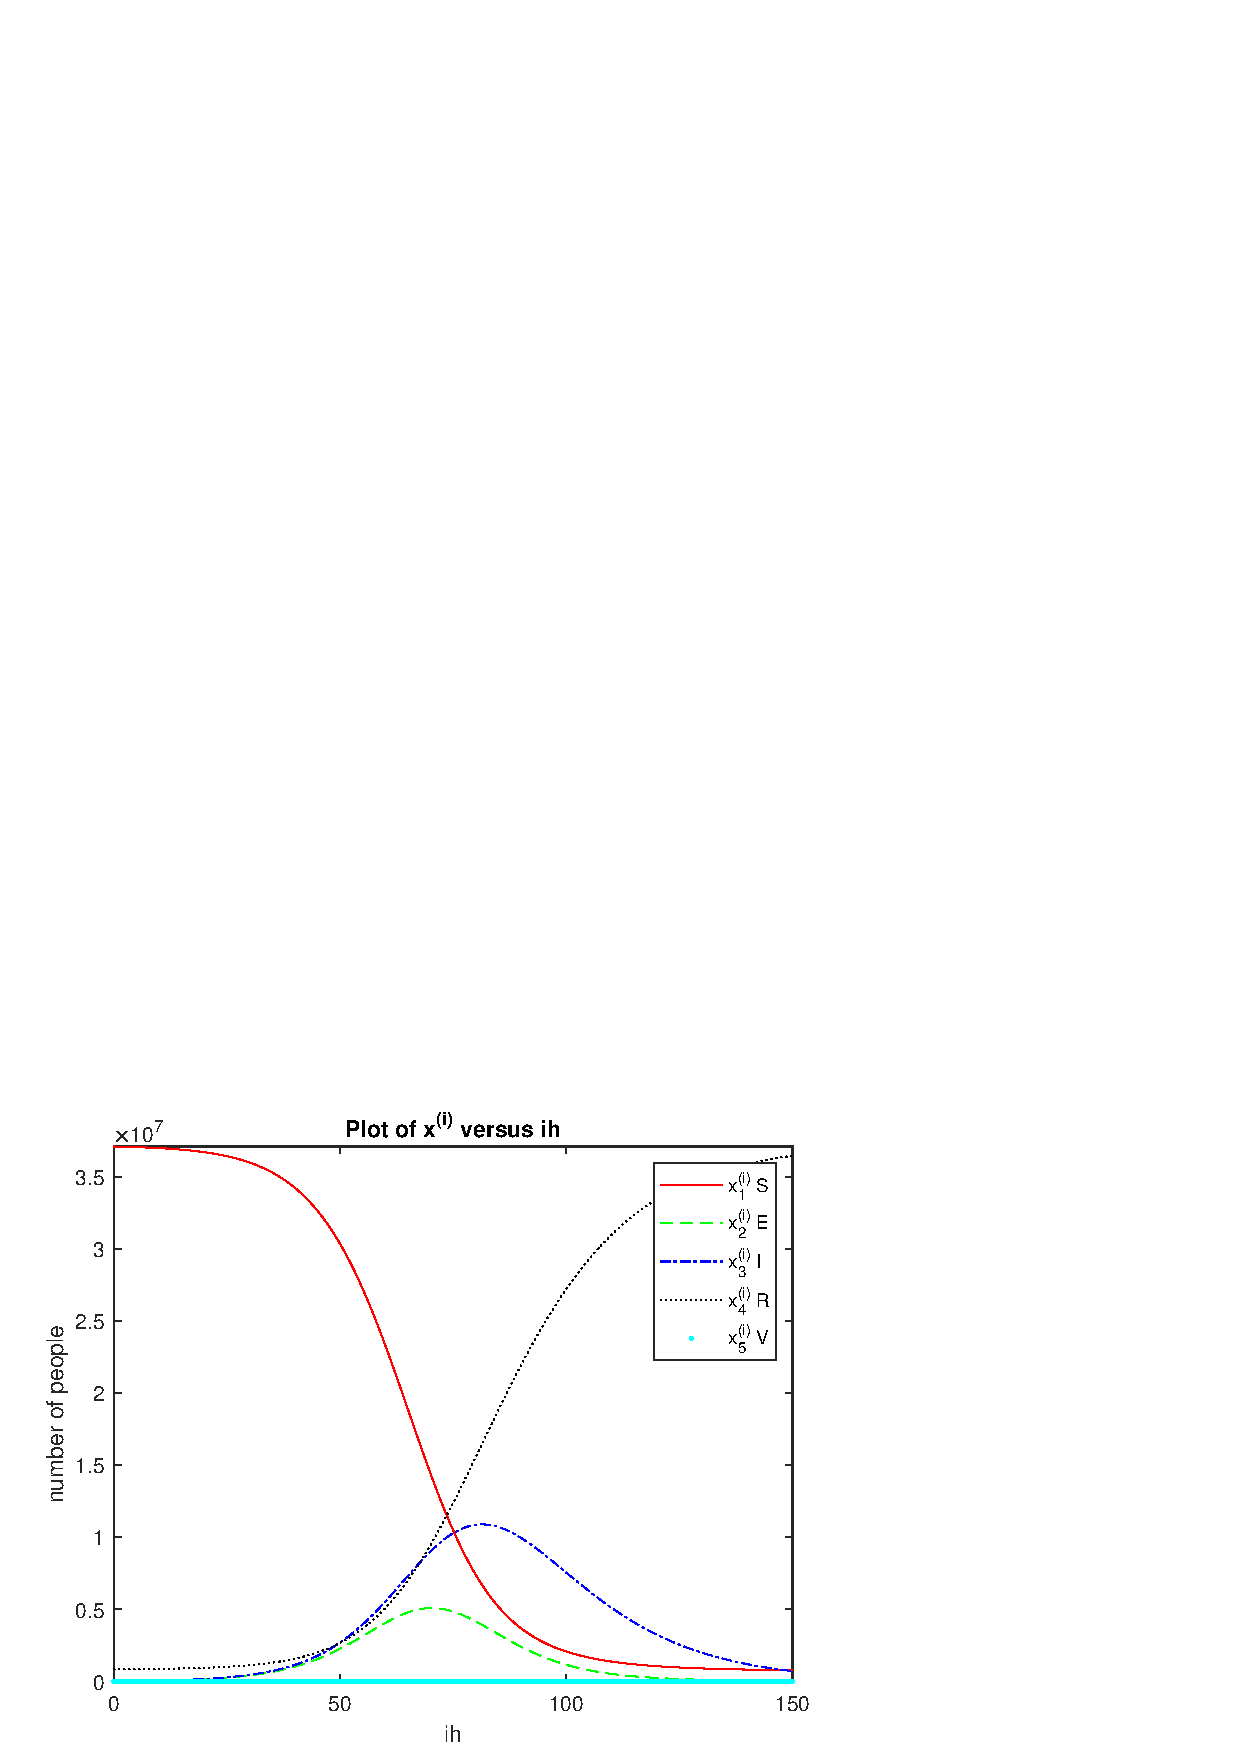
\includegraphics[width=7cm]{1c plot 1.png} }}%
    \qquad
    \subfloat[\centering number of persons in each condition each day in case d ]{{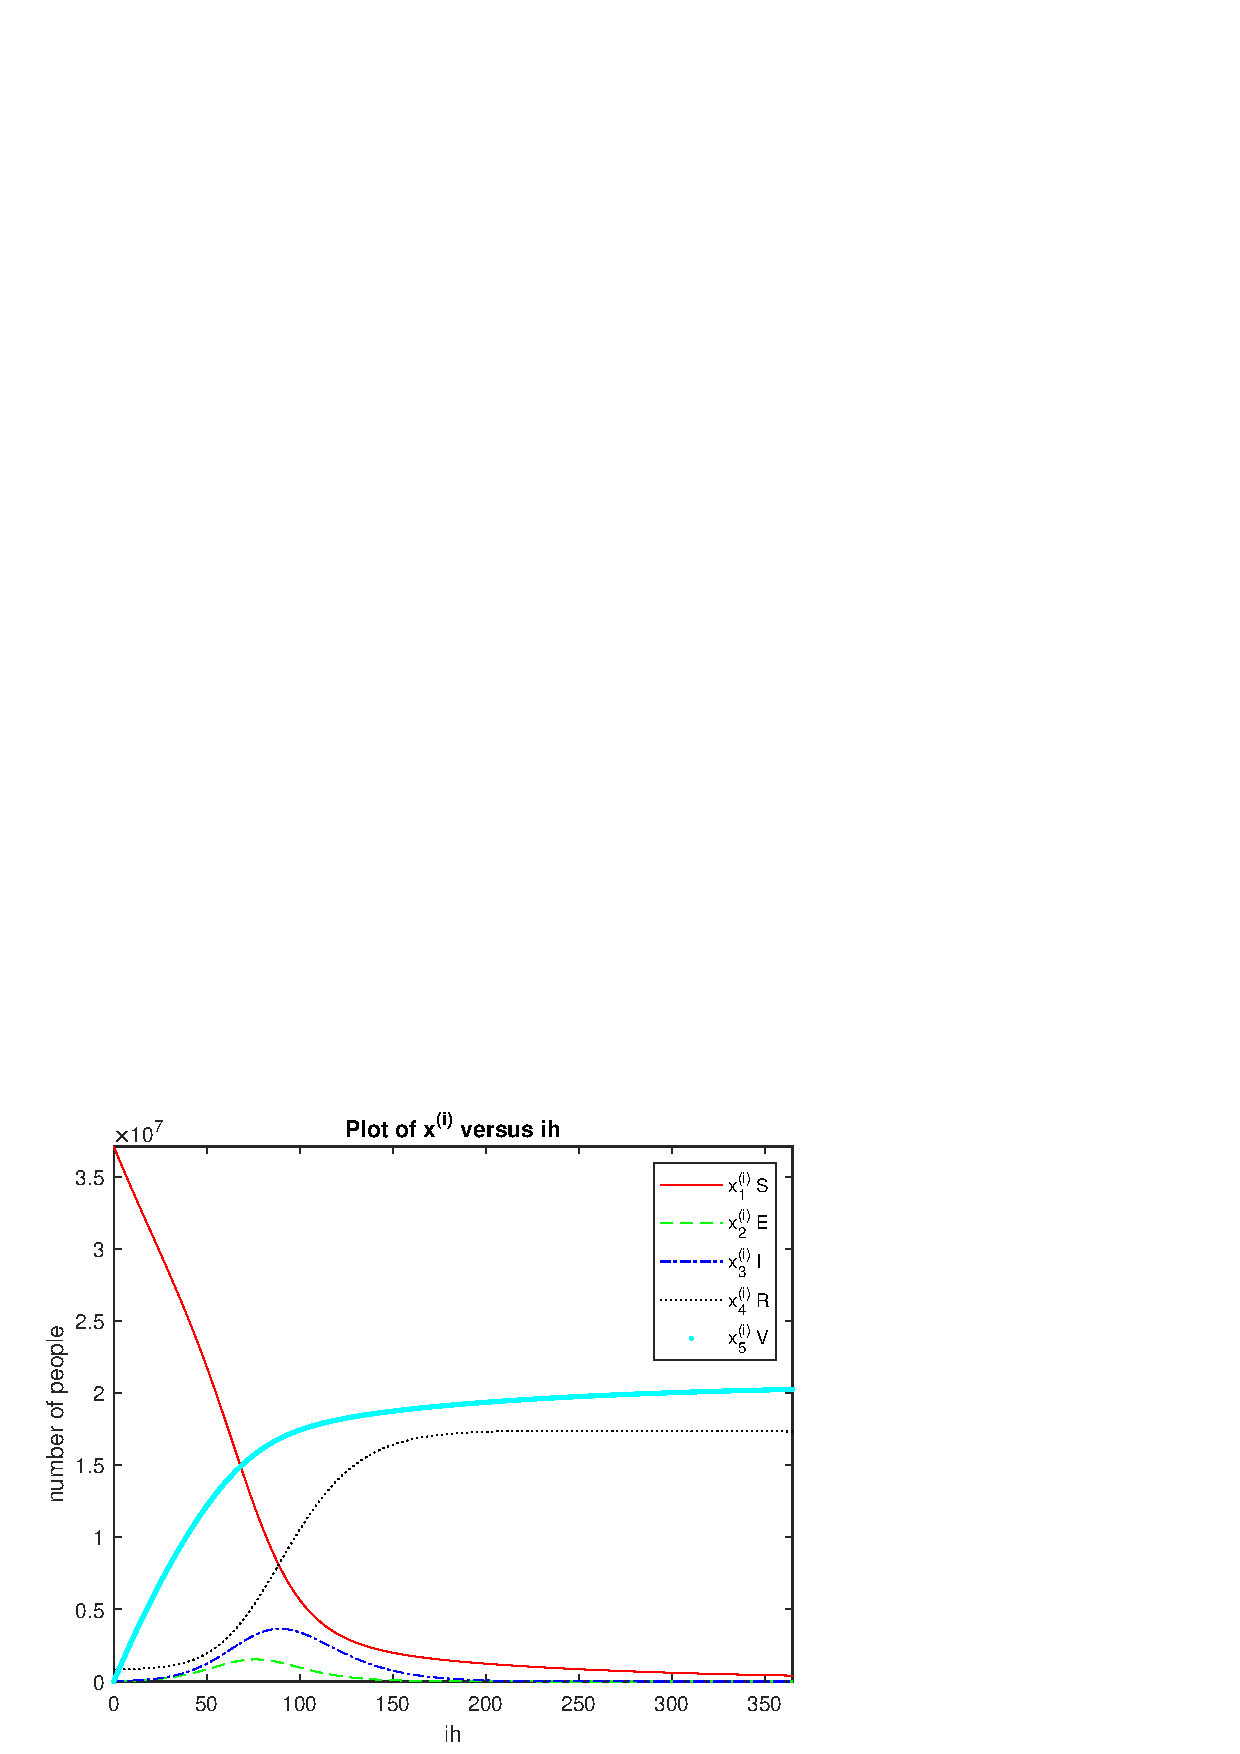
\includegraphics[width=7cm]{1d plot 1.png} }}
    \caption{2 }
    \label{fig:example}
\end{figure}\\

\begin{figure}[H]
    \centering
    \subfloat[\centering number of persons in each condition at each time step in case e  ]{{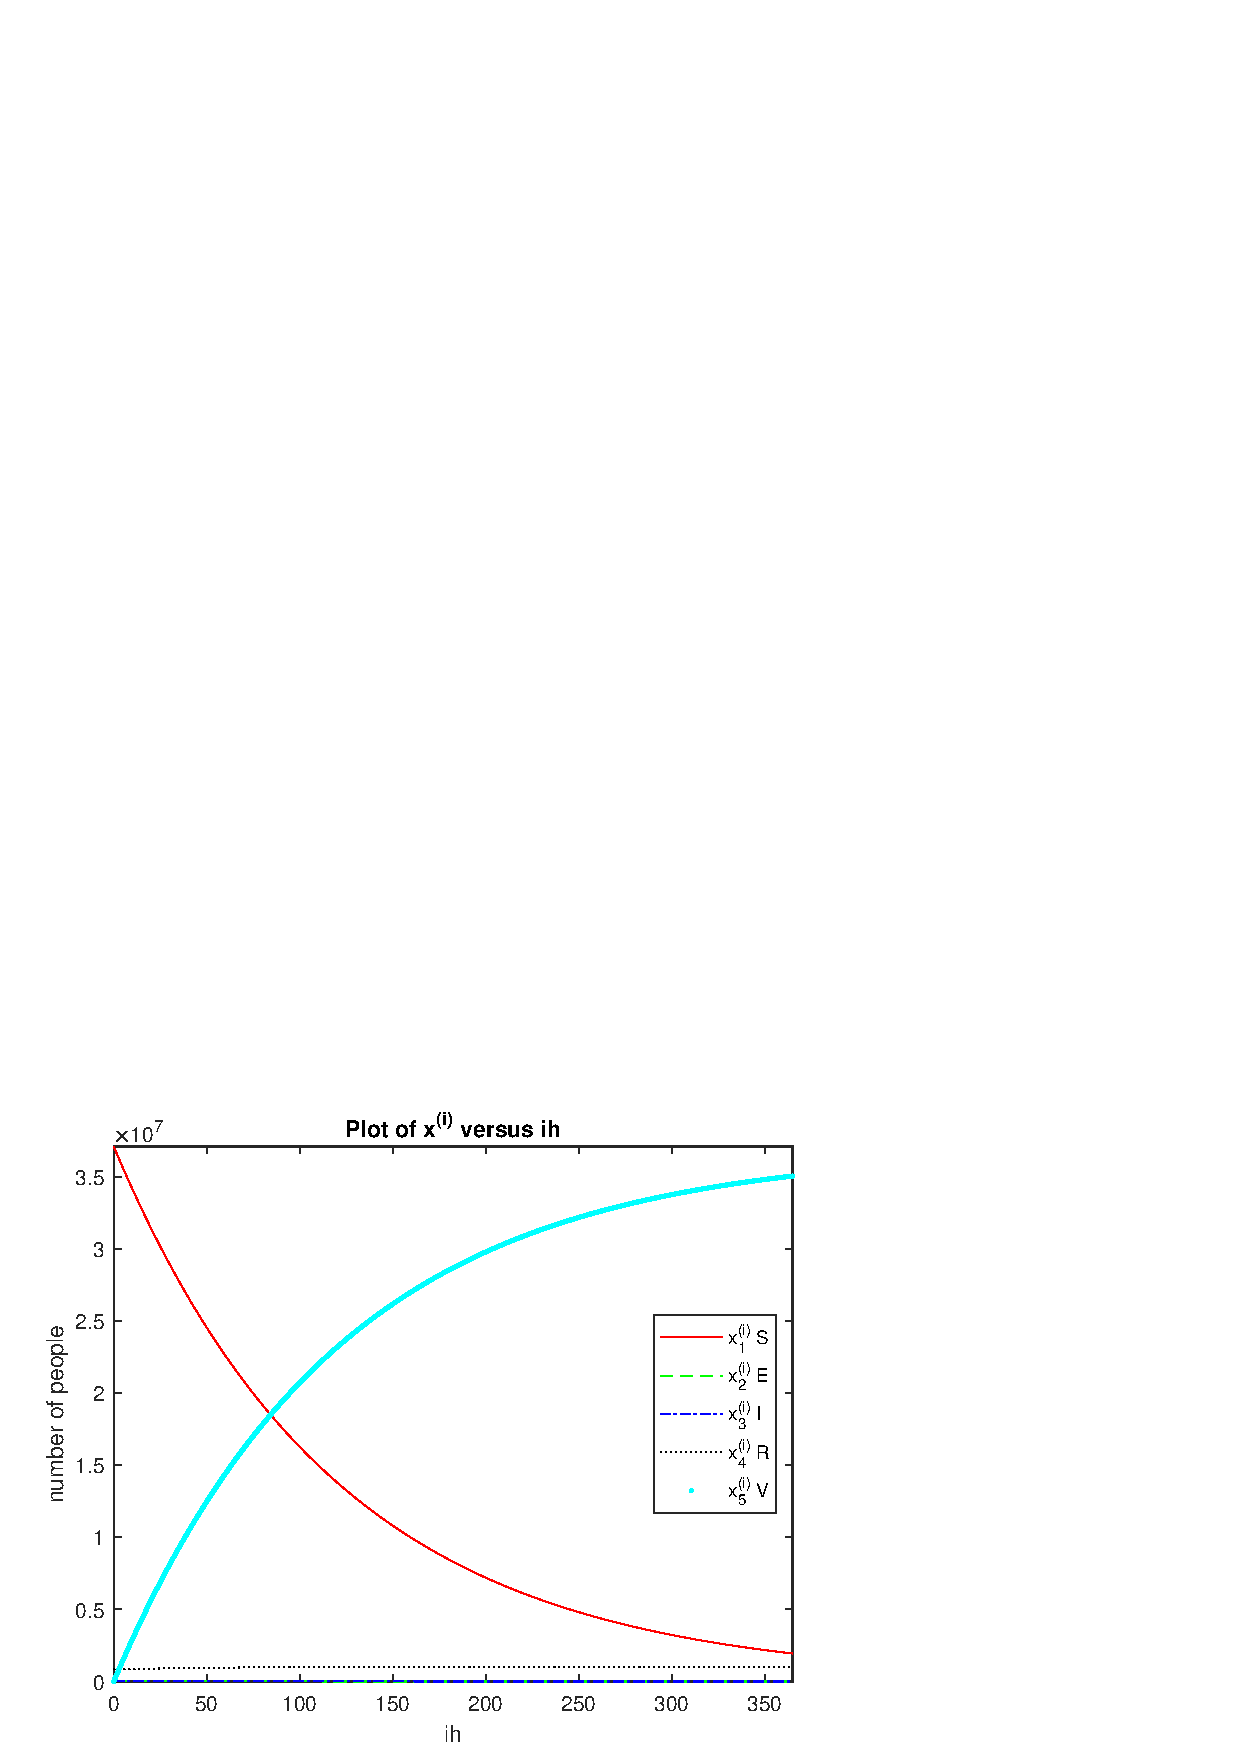
\includegraphics[width=6cm]{1e plot 1.png} }}%
    \qquad
    \subfloat[\centering number of exposed and infected persons each day in case e ]{{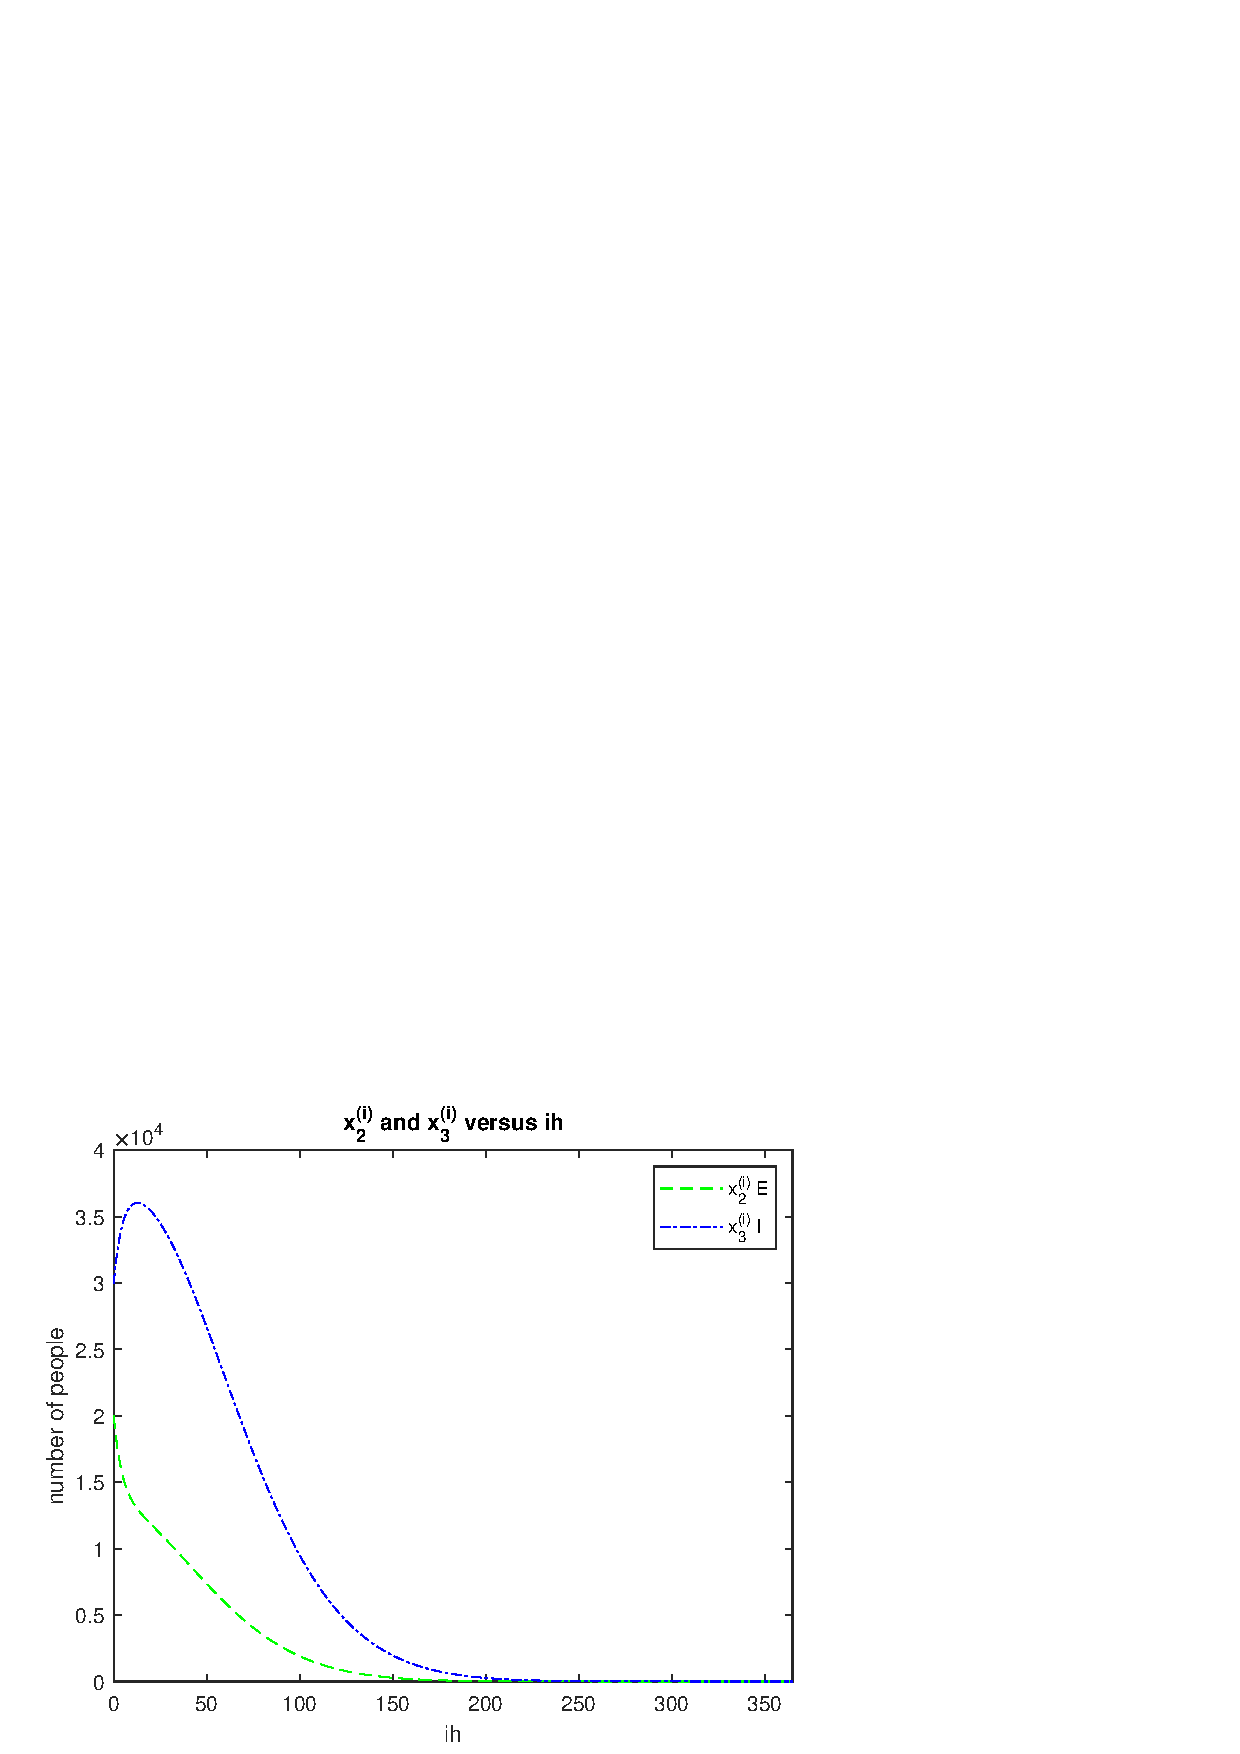
\includegraphics[width=6cm]{1e plot 3.png} }}
    \caption{comparison between case c and d }
    \label{fig:example}
\end{figure}


\begin{figure}[H]
\minipage{0.32\textwidth}
  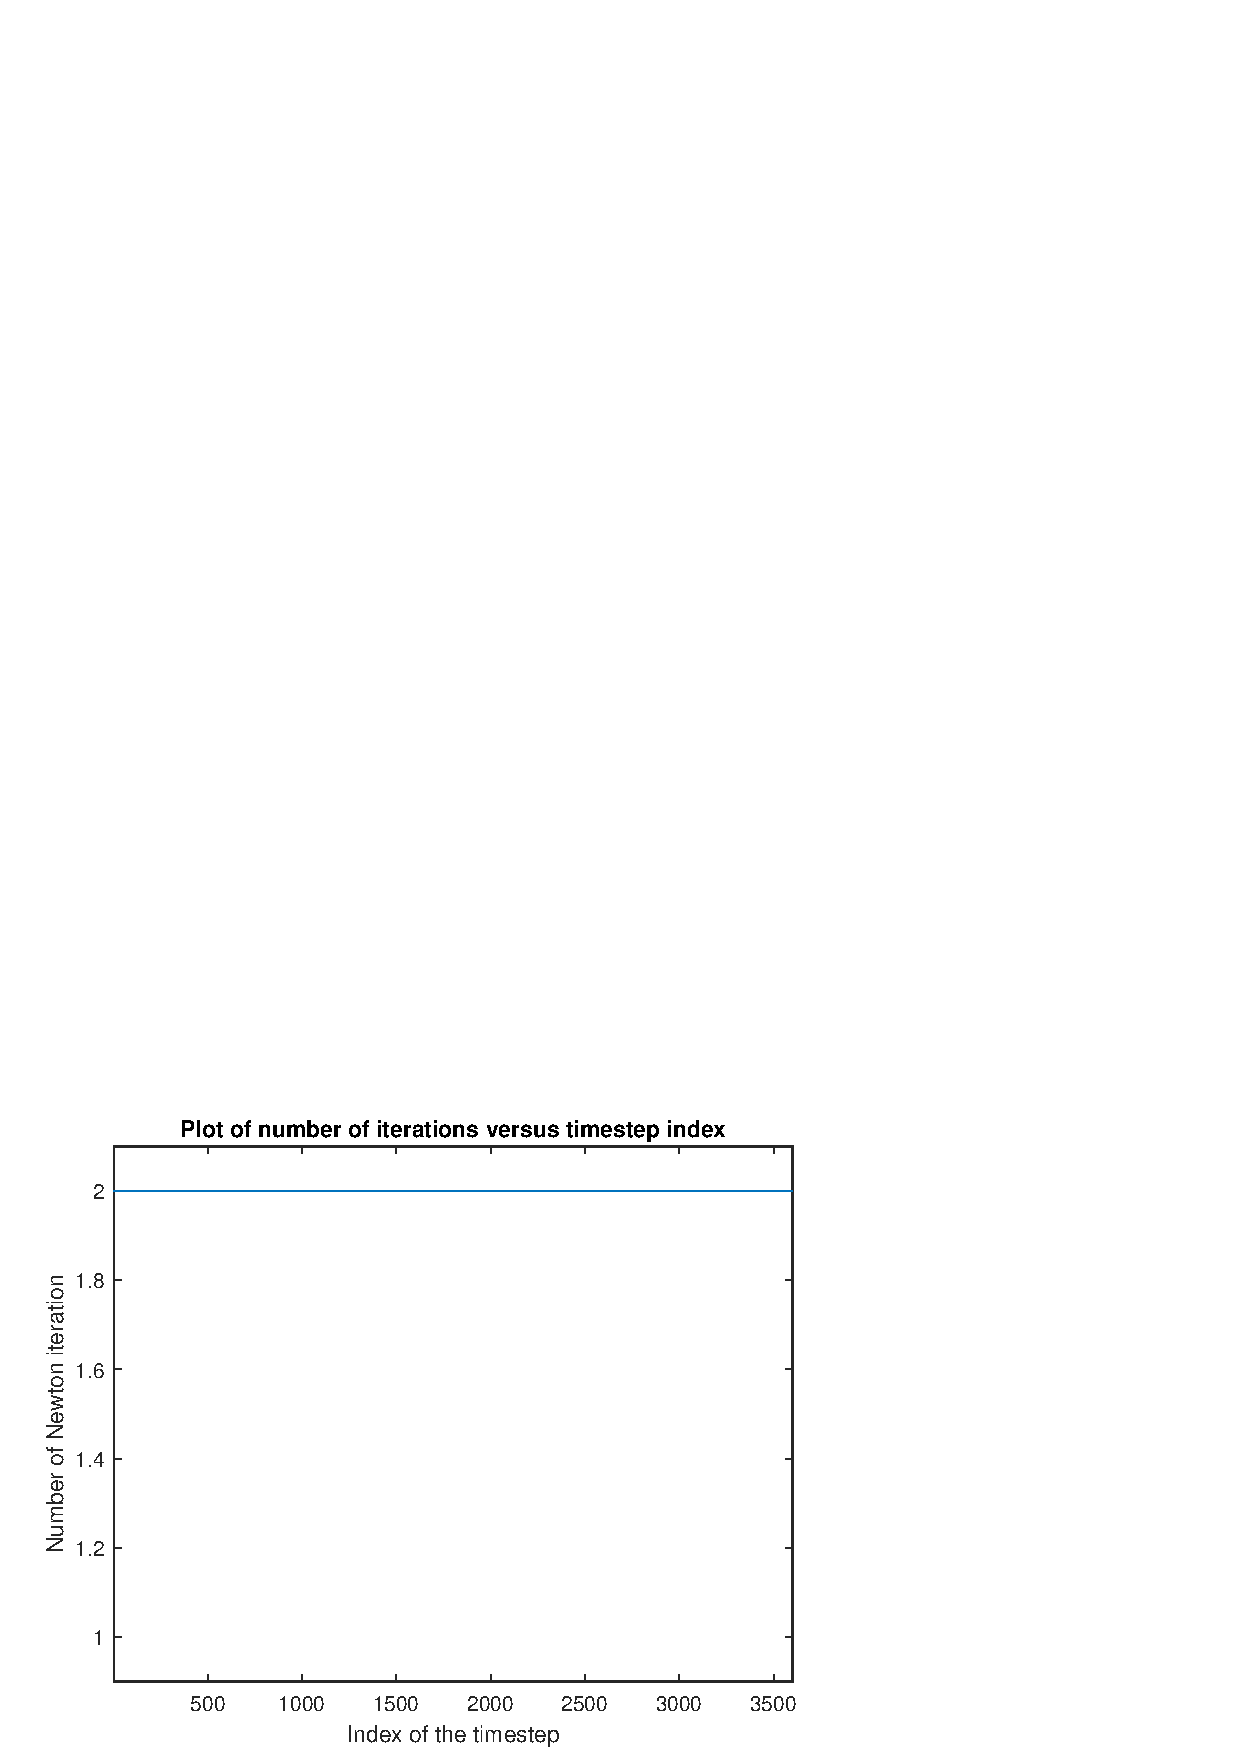
\includegraphics[width=\linewidth]{1c plot 2.png}
  \caption{number of iterations in case c}\label{fig:awesome_image1}
\endminipage\hfill
\minipage{0.32\textwidth}
  \includegraphics[width=\linewidth]{1d plot 2.png}
  \caption{number of iterations in case d}\label{fig:awesome_image2}
\endminipage\hfill
\minipage{0.32\textwidth}%
  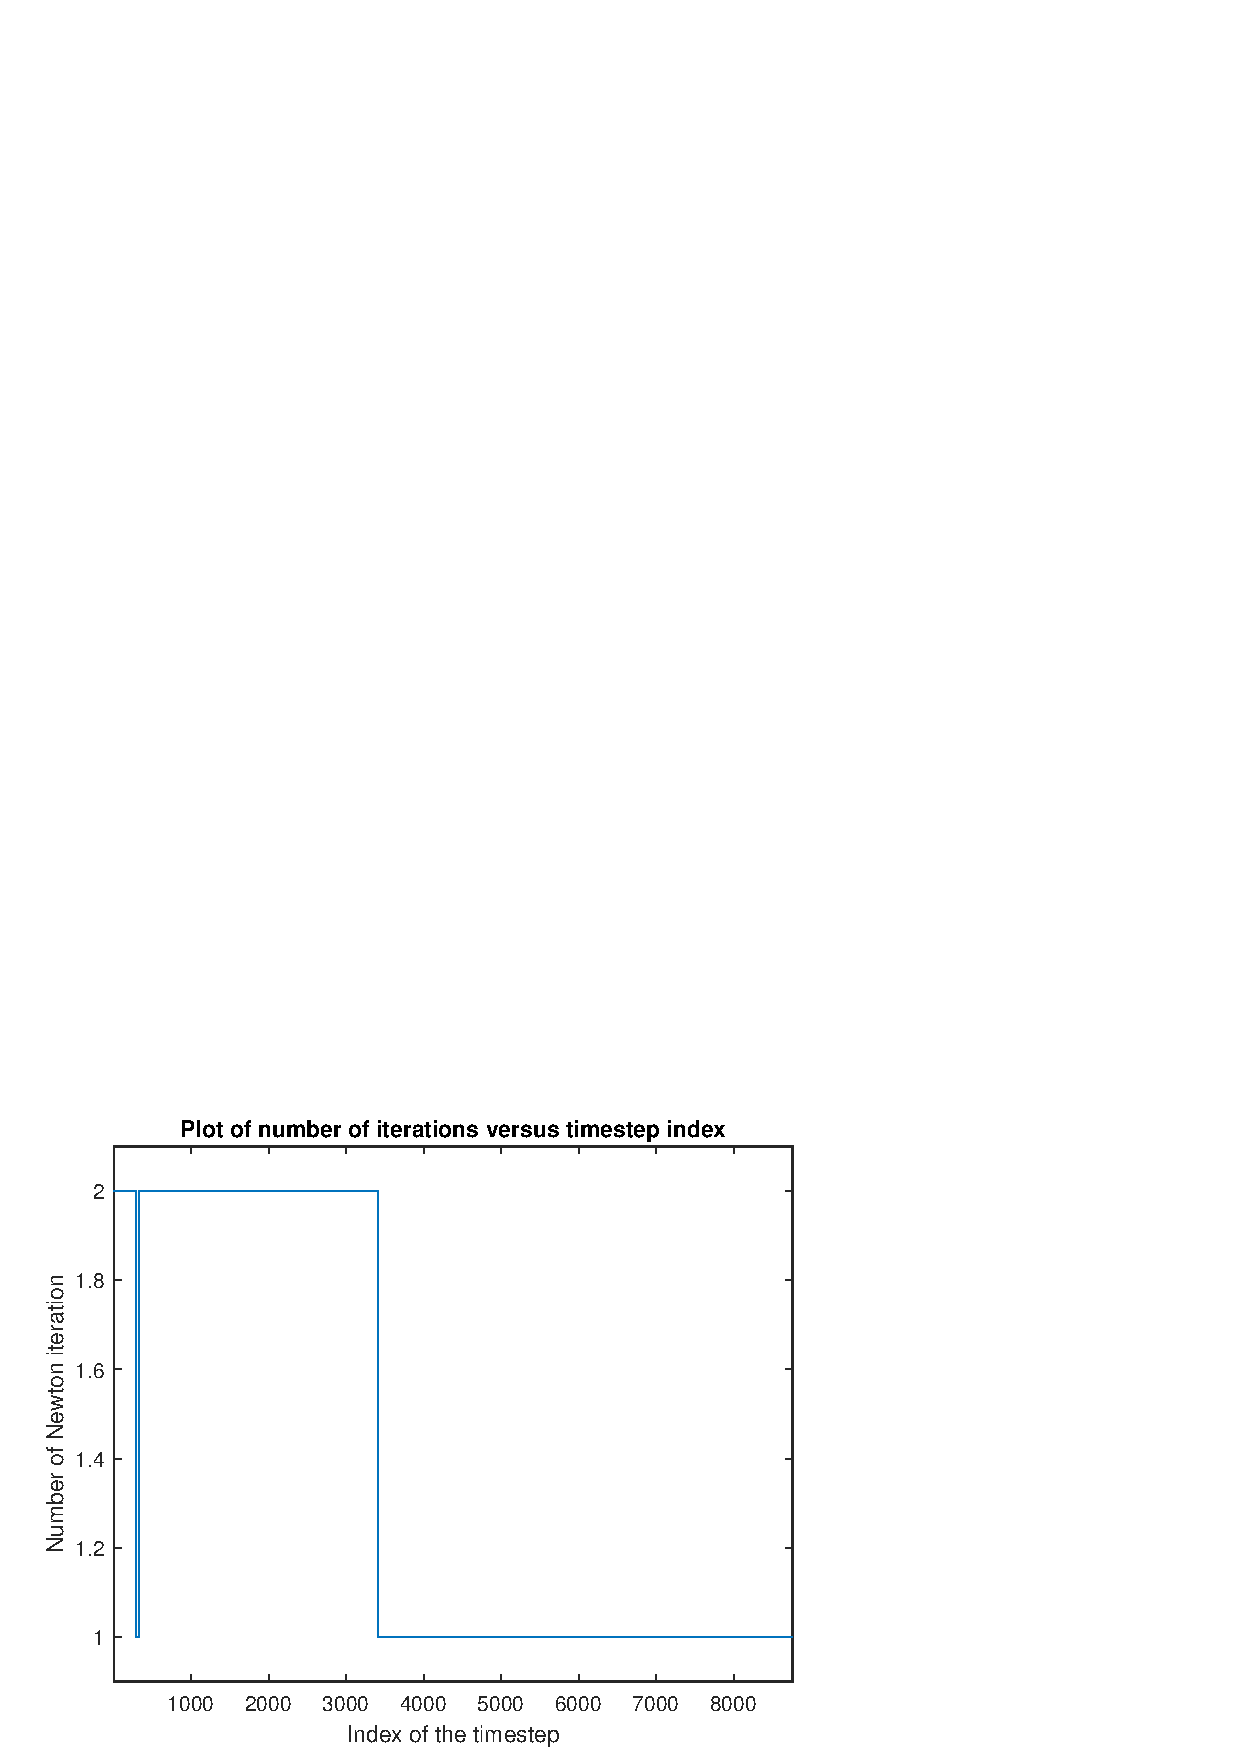
\includegraphics[width=\linewidth]{1e plot 2.png}
  \caption{number of iterations in case e}\label{fig:awesome_image3}
\endminipage
\end{figure}

\textbf{Comments:}

1. Comparing case c and d, the only difference is whether the vaccination is received or not. From the plots, the number of susceptible persons with vaccination decrease in a similar rate, but earlier than the counterpart. Also, less exposed people will get infectious and the number of infected people converges down to zero also faster if vaccination is running. The maximum number of infected people will be decreases by one order of magnitude(x10). Vaccination is definitely helpful to flatten the curve and get more people immune. At the end of the day, the number of people immune(R+V) is nearly the same.

2. The part e illustrates the case when the vaccination is running and the transmission rate is 4 times smaller than before. Then the number of vaccinated people will be increasing at a high speed as well as a considerable drop in the number of susceptible people along the time. Moreover, the maximum infection occurs at a very early time(day 12) with only less than 40 thousands people. But the rate of the susceptibles decreased is smaller than the case d. The case d reaches $0.5x10^7$ nearly 200 days faster than e.

\section{Q2}

(a)

Since $f(x)=xsin(x)-1=0 \iff sin(x)=\frac{1}{x}, \ x\neq0$, the intersection points of these two functions denote the root of $f(x)=0$. Graphically, there are two intersection points in $[0,\pi]$, so \textbf{two} roots in $[0,\pi]$.

\includegraphics[width=150mm,scale=0.5]{2a.png}

(b)

$f(x)=xsin(x)-1$ is continuous in $[\frac{\pi}{4},\frac{\pi}{2}]$ by basic properties of continuity, and since$f(\frac{\pi}{4})=\frac{\pi}{4}*\frac{\sqrt{2}}{2}-1 \approx 0.555-1 <0$ and $f(\frac{\pi}{2})=\frac{\pi}{2}-1=\frac{\pi-2}{2}>0$, by the \textbf{Bolzano existence theorem}, there exists at least one root in $(\frac{\pi}{4},\frac{\pi}{2})$. Also, $f'(x) = sinx+xcosx \Rightarrow f''(x)=cosx+cosx-xsinx=2cosx-xsinx$.

Consider$f''(x)=0 \Rightarrow 2cosx=xsinx \Rightarrow tanx = \frac{2}{x} \Rightarrow x_0 \approx 1.077$. 

Therefore, $$x \in (\frac{\pi}{4},x_0), f''(x)>0 \Rightarrow f'(x) \ increasing$$\\ $$x \in (x_0, \frac{\pi}{2}), f''(x)<0 \Rightarrow f'(x) \ decreasing$$ Notice that $f'(\frac{\pi}{2})=1>0$, $f'(\frac{\pi}{4}) = \frac{\sqrt{2}}{2}(1+\frac{\pi}{4})>0$, then we conclude $f'(x)>0 \ \forall x \in (\frac{\pi}{4},\frac{\pi}{2}) \Rightarrow f'(x) \neq 0 \forall x \in [\frac{\pi}{4},\frac{\pi}{2}]$.

Since the limit exists and $f(x)$ is differentiable in $(\frac{\pi}{4},\frac{\pi}{2})$, by \textbf{theorem 3}, f has a unique root in $[\frac{\pi}{4},\frac{\pi}{2}]$.

(c)

$f(x)=0 \iff xsinx-1=0 \iff xsinx=1 \iff x=\frac{1}{sinx} \iff x = g(x)$\\
When $x^*$is the unique root of $f(x)=0$ in $[\frac{\pi}{4},\frac{\pi}{2}]$, $x^*$is also the unique fixed point of g(x) in $[\frac{\pi}{4},\frac{\pi}{2}]$.

(d)

$g(x)=\frac{1}{sinx}$ is continuous in $[\frac{\pi}{4},\frac{\pi}{2}]$ by basic properties of continuity. Also, $g'(x)=\frac{-cosx}{sin^2 x} \leq 0 \ in [\frac{\pi}{4},\frac{\pi}{2}] \Rightarrow$ g(x) decreasing in $[\frac{\pi}{4},\frac{\pi}{2}]$ $\Rightarrow g(x)_{max} = g(\frac{\pi}{4})=\sqrt{2} \ and \ g(x)_{min}=1$.

Therefore, $\frac{\pi}{2}>\sqrt{2}>1>\frac{\pi}{4}  \Rightarrow g(x) \in [\frac{\pi}{4},\frac{\pi}{2}] \ \forall x\in[\frac{\pi}{4},\frac{\pi}{2}]$. By \textbf{Theorem 2}, there exists at least one fixed point in $[\frac{\pi}{4},\frac{\pi}{2}]$.

For contraction, $|g'(x)|=|\frac{cosx}{sin^2 x}| \leq \frac{cos(\frac{\pi}{4})}{sin^2 (\frac{\pi}{2})}=\frac{\sqrt{2}}{2}<1$, so g is a contraction by taking $\lambda=\frac{\sqrt{2}}{2}$.

By \textbf{Theorem 4b}, g has a unique fixed point $x^*$ in $[\frac{\pi}{4},\frac{\pi}{2}]$, and $\forall x^{(0)} \in [\frac{\pi}{4},\frac{\pi}{2}]$, the iteration $x^{k+1}=g(x^{k})$ converges to $x^*$. 

Take $I=[\frac{\pi}{4},\frac{\pi}{2}]$, check $|I|=\frac{\pi}{4}>\frac{\pi}{6}$ and $x^* \in [\frac{\pi}{4},\frac{\pi}{2}]$, which satisfies the requirement.

(e)

Given g has a fixed point $x^*$ and the iteration $x^{k+1}=g(x^{k})$ converges to  $x^*$ according to part (d), $g'(x)=\frac{-cosx}{sin^2 x}=0$ in $[\frac{\pi}{4},\frac{\pi}{2}]$ only if $x=\frac{\pi}{2}$, but $x^* \neq \frac{\pi}{2}$. As a result, $g'(x^*)\neq 0$.

Applying \textbf{Theorem 6}, the rate of convergence $\beta=1$.

(f)

We have already shown this in (d), so \textbf{skip}.

(g)

With initial guess $x^{(0)}=\frac{\pi}{2}$, recall the formula of Newton's iteration $$ x^{(1)}=x^{(0)}-\frac{f(x^{(0)})}{f'(x^{(0)})}=\frac{\pi}{2}-\frac{\frac{\pi}{2}-1}{sin(\frac{\pi}{2})+\frac{\pi}{2}cos(\frac{\pi}{2})}=\frac{\pi}{2}-\frac{\frac{\pi}{2}-1}{1}=\frac{\pi}{2}-\frac{\pi}{2}+1=1$$. 

Therefore, $x^{(1)}=1$.

\section{Q3}

(a)

For the function $f(x) = e^{-x}$, given base points $x_0=-1$ and $x_1=1$, $f_0 = e$ and $f_1 = e^{-1}$,so $f[x_0,x_1]=\frac{f_1-f_0}{x_1-x_0} = \frac{e^{-1}-e}{2}$. The NDD table is constructed as follows:

\begin{center}
\begin{tabular}{ |c c|c| } 
\hline
\multirow -1 & e & \\ 
&  & $\frac{e^{-1}-e}{2}$ \\ 
1 & e^{-1} &  \\ 
\hline
\end{tabular}
\end{center}
The interpolating polynomial $p_1(x) = f_0+f[x_0,x_1](x-x_0)=f_0+\frac{f_1-f_0}{x_1-x_0}(x-x_0) = e+\frac{e^{-1}-e}{2}(x+1) = \frac{e^{-1}-e}{2}x+\frac{e^{-1}+e}{2}$

(b)

Given $n=1$ and $f(x) = e^{-x}$, we first verify the assumptions of the theorem: $f'(x) = -e^{-x}$ and $f''(x) = e^{-x}$. Both derivatives are continuous, so f(x) has n+1=2 continuous derivatives. Suppose $p_n(x)$ is the polynomial of degree at most 2 interpolating f at $x_0 \ and \ x_1$, then for any x, the polynomial interpolation error formula from the theorem is
\begin{equation}
\begin{aligned}
f(x)-p_n(x) &=\frac{f^{n+1}(\xi)}{(n+1)!}\Pi_{j=0}^n(x-x_j)\\
e^{-x}-p_1(x) &=\frac{e^{-\xi}}{2}(x^2-1) \\
e^{-x} - (\frac{e^{-1}-e}{2}x+\frac{e^{-1}+e}{2})&= \frac{e^{-\xi}}{2}(x^2-1)
\nonumber
\end{aligned}
\end{equation}

where $\xi$ is an unknown point in$\ ospr \{ x_0,x_1\}= (-1,1)$.

To get a bound for $|e^{-x}-p_1(x)|$ for any $x \in [-1,1]$, we first know from the theorem that \textbf{$\xi \in (-1,1)$}. We maximize$|W(x)=x^2-1|$. It's easy to notice that $|W(x)|$ reaches the minimal value at $x=0$ i.e. $W_{min}(x)=-1$, so $max_{-1\leq x \leq 1}|W(x)|=max \{|W(x)|: x=-1,x=1,x=0 \}=max \{ 0,1 \}$=1. Then, for $-1 \leq x \leq 1$, $$|e^{-x}-p_1(x)| \leq \frac{e^{-\xi}}{2}<\frac{e^{-(-1)}}{2}=\frac{e}{2}\approx 1.36$$.

To get a bound for $|e^{-x}-p_1(x)|$ for any $x \in [1,2]$, we first know $\xi \in (-1,2)$. Then, $max_{1\leq x \leq 2}|W(x)|=max \{|W(x)|: x=-1,x=1,x=0,x=2 \}=max \{ 0,1,3 \}= 3$, taking into account that $|W(2)|=3$. Therefore, for $x \in [1,2]$, $$|e^{-x}-p_1(x)|\leq \frac{3*e^{-\xi}}{2}<\frac{3e}{2}\approx 4.078$$.

(c)

The NDD table is the following:

\begin{center}
\begin{tabular}{|c c|c|c| } 
\hline
\multirow -1 & e & & \\ 
& & 1-e & \\ 
0 & 1 & & $\frac{e+e^{-1}-2}{2}$\\
& & e^{-1}-1 & \\ 
1 & e^{-1} &  & \\ 
\hline
\end{tabular}
\end{center}

Since $a_i=f[x_0,x_1,...,x_i]$,$b_i(x)=(x-x_0)(x-x_1)...(x-x_{i-1})$ and $i=2$ in this case, $$p_2(x)=\sum_{j=0}^{2}=e+(1-e)(x+1)+\frac{e+e^{-1}+2}{2}(x+1)(x-0)=1+(\frac{e^{-1}-e}{2})x+(\frac{e^{-1}+e}{2}-1)x^2$$

(d)

The polynomial interpolation error formula is 
\begin{equation}
\begin{aligned}
f(x)-p_n(x) &=\frac{f^{n+1}(\xi)}{(n+1)!}\Pi_{j=0}^n(x-x_j)\\
e^{-x}-p_2(x) &=\frac{-e^{-\xi}}{3!}x(x+1)(x-1) \\
e^{-x} - p_2(x) &= \frac{-e^{-\xi}}{6}(x^3-x)
\nonumber
\end{aligned}
\end{equation}

To get a bound for $|e^{-x}-p_2(x)|$ for any $x \in [-1,1]$, we first know from the theorem that \textbf{$\xi \in (-1,1)$}. Then, to maximize$|W(x)|=x^3-x$, we have $W'(x)=3x^2-1 \Rightarrow W''(x)=6x$. Note that $W'(x)=0 \Rightarrow x= \frac{\sqrt{3}}{3} or x = -\frac{\sqrt{3}}{3}$. From the quadratic form of the derivative, $$x \in (-1,-\frac{\sqrt{3}}{3}),W'(x)>0 \Rightarrow W(x) \ increasing$$\\ $$x \in (-\frac{\sqrt{3}}{3},\frac{\sqrt{3}}{3}),W'(x)<0 \Rightarrow W(x) \ decreasing$$

$$x \in (\frac{\sqrt{3}}{3},1),W'(x)>0 \Rightarrow W(x) \ increasing$$ 

so $max_{-1\leq x \leq 1}|W(x)|=max \{|W(x)|: x=-1,x=1,x= -\frac{\sqrt{3}}{3}, x=\frac{\sqrt{3}}{3} \}=max \{ 0,\frac{2}{3\sqrt{3}} \}=\frac{2}{3\sqrt{3}}=\frac{2\sqrt{3}}{9}$. Then, for $-1 \leq x \leq 1$, $$|e^{-x}-p_1(x)| \leq \frac{e^{-\xi}}{6}*\frac{2\sqrt{3}}{9}<\frac{e^{-(-1)}}{6}=\frac{e}{6}*\frac{2\sqrt{3}}{9}=\frac{\sqrt{3}e}{27}$$.

To get a bound for any $x\in [1,2]$, we first know from the theorem that $\xi \in (-1,2)$. Then, to maximize $|W(x)|$, we've shown that $W(x)$ will be increasing whenever $x> \frac{\sqrt{3}}{3}$, so $max_{-1\leq x \leq 1}|W(x)|=max \{|W(x)|: x=-1,x=1,x= -\frac{\sqrt{3}}{3}, x=\frac{\sqrt{3}}{3} ,x=2 \}=max \{ 0,\frac{2}{3\sqrt{3}},6 \}=6$.

Therefore, for $1 \leq x \leq 2$,$$|e^{-x}-p_1(x)| \leq \frac{e^{-\xi}}{6}*6<e^{1}=e$$ .

(e)

Given the Taylor polynomial of $e^x = \sum_{n=0}^{\infty}\frac{x^n}{n!}$ about x = 0, $f(x)=e^{-x}=\sum_{n=0}^{\infty}\frac{(-x)^n}{n!}$, so $t_1(x)=1-x$ and $t_2(x)=1-x+\frac{x^2}{2}$. The MATLAB script, plots and output are the followings:

\begin{figure}[H]
    \centering
    \subfloat[\centering Polynomial Approximations and True Values  ]{{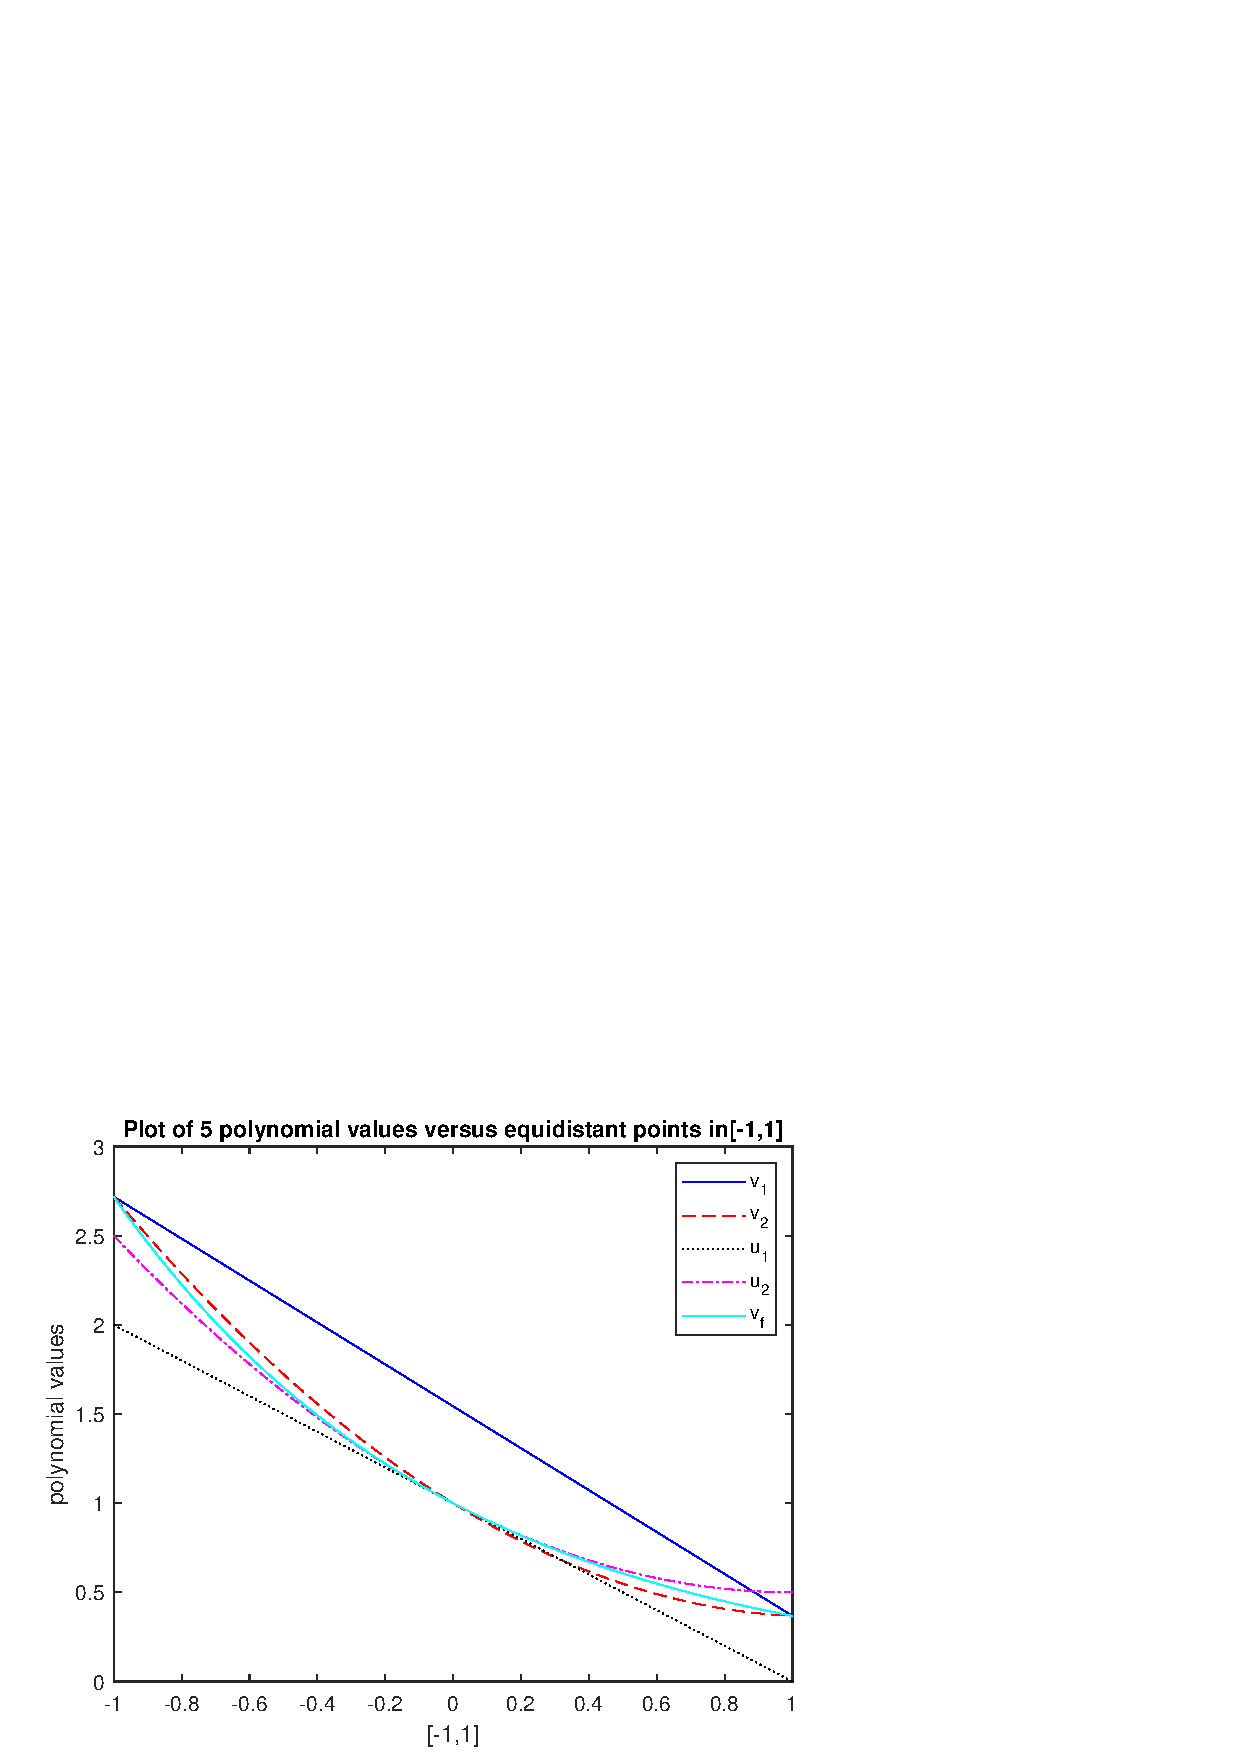
\includegraphics[width=11cm]{2e plot 1.png} }}%
    \qquad
    \subfloat[\centering Approximation Errors ]{{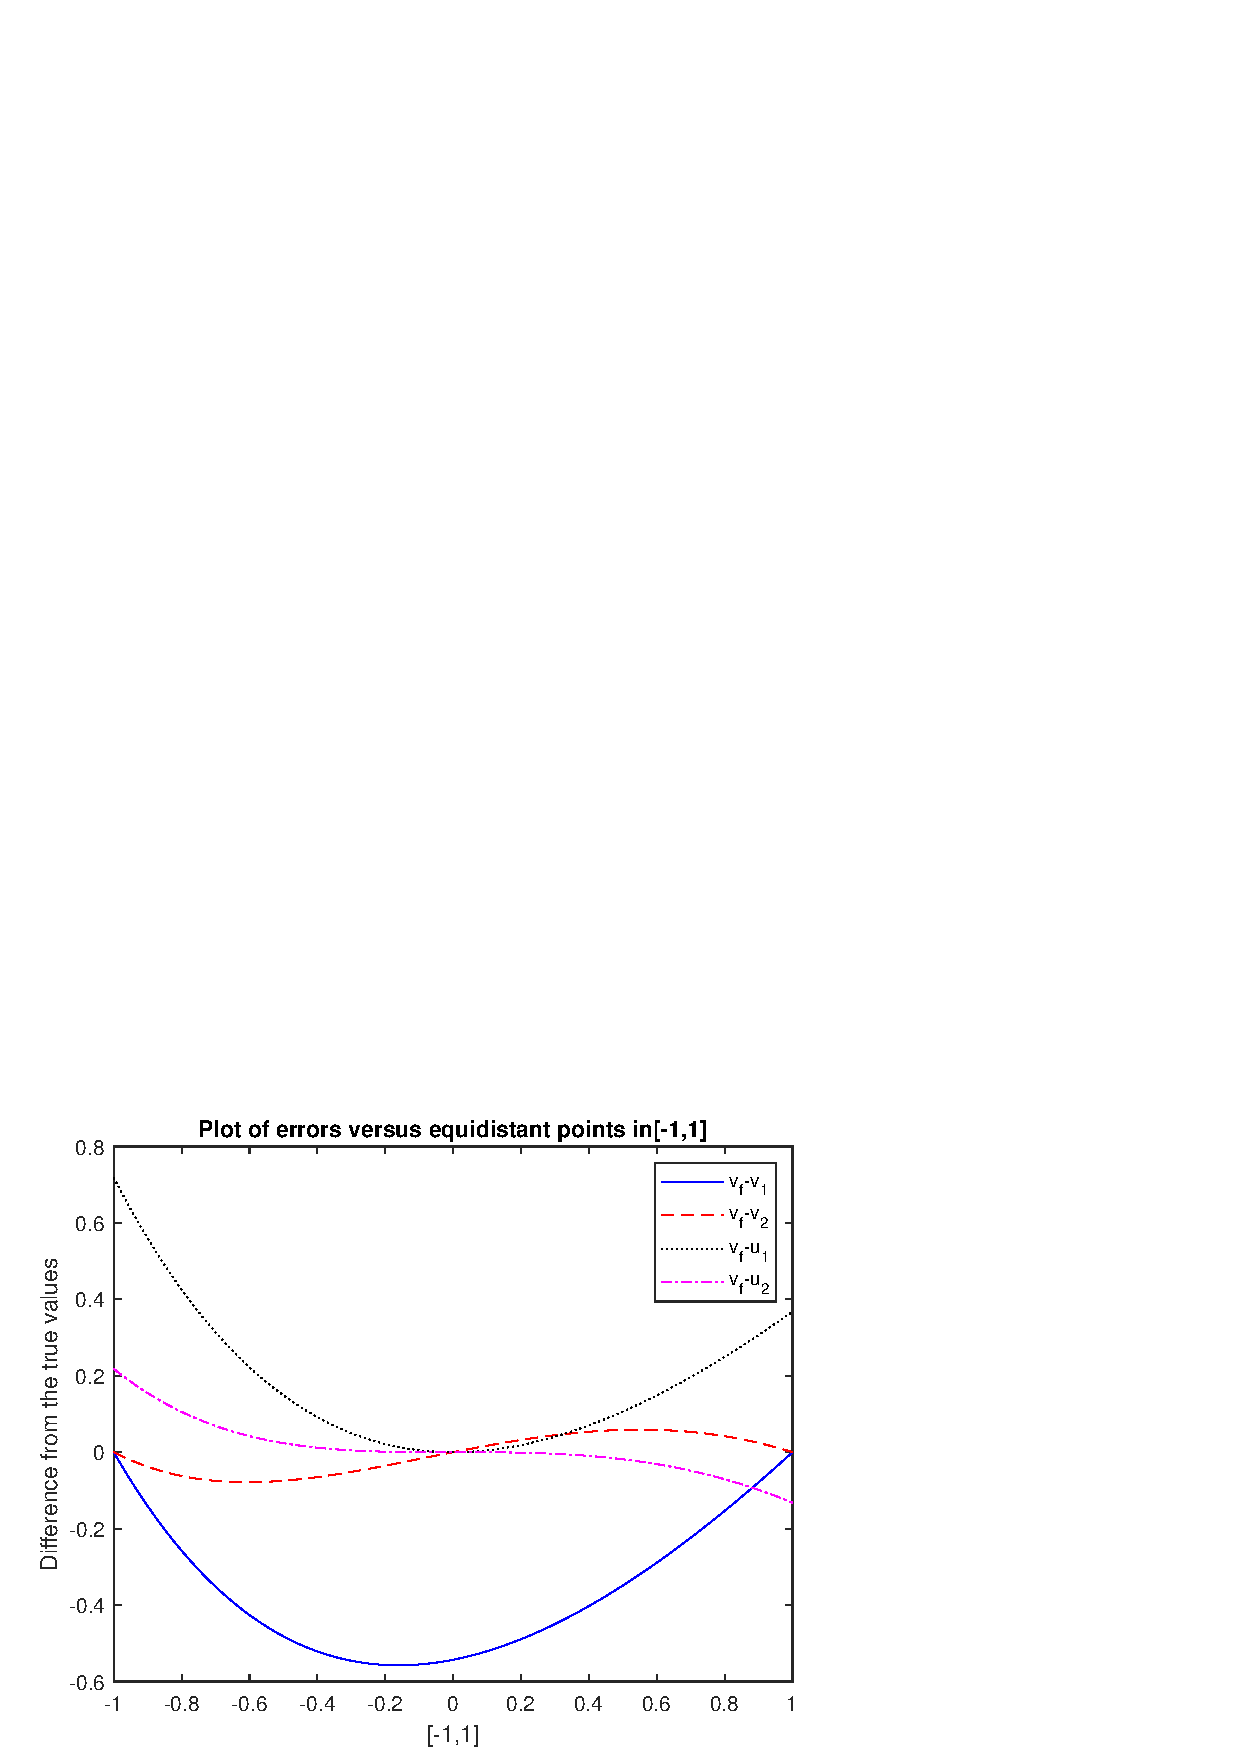
\includegraphics[width=11cm]{2e plot 2.png} }}
    \caption{2 Polynomial Approximations to $f(x)=e^{-x}$}
    \label{fig:example}
\end{figure}\\

\begin{lstlisting}
%(e)
x1 = [-1,1];
y1 = [exp(1),1/exp(1)];
x2 = [-1,0,1];
y2 = [exp(1),1,1/exp(1)];
p1 = polyfit(x1,y1,1);
p2 = polyfit(x2,y2,2);
fprintf('p_1(x) interpolation\n');
fprintf('%3f %3f \n',polyval(p1,x1));
fprintf('p_2(x) interpolation\n');
fprintf('%3f %3f %3f \n',polyval(p2,x2));

x = linspace(-1,1,100);
u1 = 1-x;
u2 = 1-x + 0.5*x.^2;
v1 = polyval(p1,x);
v2 = polyval(p2,x);
vf= exp(-x);
fprintf('max absolute values of errors\n')
fprintf('vf-v1:%3f vf-v2: %3f vf-u1: %3f vf-u2: %3f\n',max(abs(vf-v1)),max(abs(vf-v2)),max(abs(vf-u1)),max(abs(vf-u2)))

% the first plot
plot(x,v1,'-b',x,v2,'--r',x,u1,':black',x,u2,'-. m',x,vf,'c-')
legend('v_1','v_2','u_1','u_2','v_f')
xlabel('[-1,1]')
ylabel('polynomial values')
title('Plot of 5 polynomial values versus equidistant points in[-1,1]')

% the second plot
plot(x,vf-v1,'-b',x,vf-v2,'--r',x,vf-u1,':k',x,vf-u2,'-.m')
legend('v_f-v_1','v_f-v_2','v_f-u_1','v_f-u_2')
xlabel('[-1,1]')
ylabel('Difference from the true values')
title('Plot of errors versus equidistant points in[-1,1]')
\end{lstlisting}\\
\textbf{Output}:\\
$p_1(x)$ interpolation:\\
2.718282 0.367879 \\
$p_2(x)$ interpolation:\\
2.718282 1.000000 0.367879\\ 
max absolute values of errors:\\
vf-v1:0.557545 vf-v2: 0.078491 vf-u1: 0.718282 vf-u2: 0.218282\\
\textbf{Comments on the results:}

For a small number of data points, more points used for interpolation, smaller errors there would be for both Taylor expansion and polynomial interpolation. 

To be more specific, from the plots, $t_2(x)$ lies closer to the true function f than $t_1(x)$ and both are tangent to f at x=0. Similarly, the interpolating polynomial $p_2(x)$ as a curve fits nicer than $p_1(x)$, a straight line with only two data points.

From the error plot, we can say that with more equidistant data points, the error bounds for both approximation methods get smaller, or visually speaking, flatter.

\section{Q4}

The added script is the following:

\begin{lstlisting}
a = -1; b = 2;
xe = linspace(a, b, 1000);
ye = exp(-xe);

disp(['interval (' num2str(a) ',' num2str(b), ')'])
disp('  n    err poly   err lin_spl')
for nn = 1:6
    n = 2^nn;
    xi = linspace(a, b, n+1);
    yi = exp(-xi);
    py = polyfit(xi,yi,n);
    yp = polyval(py,xe); % polynomial interpolant at (xi, yi), evaluated at xe
    yl = interp1(xi,yi,xe,'linear'); % linear spline interpolant at (xi, yi), evaluated at xe
    ep = max(abs(yp-ye)); % infinity error norm of polynomial interpolant
    el = max(abs(yl-ye)); % infinity error norm of linear spline interpolant
    fprintf('%3d %12.3e %12.3e\n', n, ep, el);
end

fprintf('\n')
disp(['interval (' num2str(a) ',' num2str(b), ')'])
disp('    n   err lin_spl err cub_spl')
for nn = 4:14
    n = 2^nn;
    xi = linspace(a, b, n+1);
    yi = exp(-xi);
    yl = interp1(xi,yi,xe,'linear'); % linear spline interpolant at (xi, yi), evaluated at xe
    yc = spline(xi,yi,xe); % cubic spline interpolant at (xi, yi), evaluated at xe
    el(nn) = max(abs(yl-ye)); % infinity error norm of linear spline interpolant
    ec(nn) = max(abs(yc-ye)); % infinity error norm of cubic spline interpolant
    fprintf('%5d %12.3e %12.3e ', n, el(nn), ec(nn));
    if (nn > 4)
        fprintf('%6.1f %6.1f\n', log(el(nn-1)/el(nn))/log(2), ...
                                 log(ec(nn-1)/ec(nn))/log(2));
    else fprintf('\n'); end
end
\end{lstlisting}

\textbf{Output}:
\begin{lstlisting}
interval (-1,2)
  n    err poly   err lin_spl
  2    1.853e-01    3.842e-01
  4    5.797e-03    1.334e-01
  8    1.453e-06    3.977e-02
 16    1.599e-14    1.089e-02
Warning: Polynomial is badly conditioned. Add points with distinct X values, reduce the degree of the polynomial, or try centering and scaling as described in
HELP POLYFIT. 
> In polyfit (line 83)
In scriptint (line 11) 
 32    1.086e-09    2.848e-03
Warning: Polynomial is badly conditioned. Add points with distinct X values, reduce the degree of the polynomial, or try centering and scaling as described in
HELP POLYFIT. 
> In polyfit (line 83)
In scriptint (line 11) 
 64    7.833e+01    7.287e-04

interval (-1,2)
    n   err lin_spl err cub_spl
   16    1.089e-02    7.831e-05 
   32    2.848e-03    5.385e-06    1.9    3.9
   64    7.287e-04    3.526e-07    2.0    3.9
  128    1.843e-04    2.258e-08    2.0    4.0
  256    4.636e-05    1.332e-09    2.0    4.1
  512    1.162e-05    8.098e-11    2.0    4.0
 1024    2.748e-06    4.912e-13    2.1    7.4
 2048    7.075e-07    3.153e-14    2.0    4.0
 4096    1.796e-07    2.220e-15    2.0    3.8
 8192    4.350e-08    4.441e-16    2.0    2.3
16384    1.091e-08    4.441e-16    2.0    0.0
\end{lstlisting}

\textbf{Comments:}

As the number of data points increases, the errors of the polynomial approximation decreases drastically for some small n but as n>16, the warnings come up and say the polynomial is badly conditioned. Also, the errors go higher again afterwards, showing an oscillatory behaviour towards the endpoints. Equidistant choice of points $x_i$ induce this issue, and this phenomenon agrees with the theory. Using Chebyshev points is more preferred.

As the number of data points increases, the errors of linear spline interpolation decreases and the error is of second order according to the second and penultimate columns of the bottom table, which also agrees with the theory.

As the number of data points increases, the errors of cubic spline interpolation decrease and the error is of fourth order except for few exceptions according to the second and the rightmost columns of the bottom table, which agrees with the theory in general. When n is extremely high e.g. n>4096, the rate of improvement starts to decrease to zero. This is not expected from the theory

\end{document}
